\documentclass[a4paper]{article}

\usepackage{a4wide}
\usepackage[latin1]{inputenc}
\usepackage[portuguese]{babel}
\usepackage{clrscode} % para os algoritmos estilo CLRS
\usepackage{graphicx} % para as imagens


\renewcommand{\baselinestretch}{1.5}
\begin{document}

% INICIO DA CAPA %%%%%%%%%%%%%%%%%%%%%%%%%%%%%%%%%%%%%%%%%%%%%%%%%%%%%%%%%%%%%%
\thispagestyle{empty}
\null
\vskip-3cm
\null
\hskip-1.9cm
\noindent
%\scalebox{0.75}{
\includegraphics{figura}}%\\
\null
\vskip0.5cm                
\begin{center}
  {\LARGE \textsc{Instituto Superior de Engenharia de Lisboa}}
  \\[1cm]
  {\huge \bf An�lise e processamento distribu�do de redes de grande dimens�o}
  \\[0.5cm]
  {\large {\bf Proposta de Projecto}}
  
  {\large
    \ifcase\month\or Janeiro\or Fevereiro\or Mar\c{c}o\or Abril\or Maio\or
      Junho\or Julho\or Agosto\or Setembro\or Outubro\or Novembro\or Dezembro
    \fi
    \space de\space\the\year}
  \\[0.5cm]
  \begin{minipage}[t]{7cm}
    \flushleft
    \textsc{Orientadores:}
    
    C�tia Vaz (ISEL)
    
    Alexandre Francisco (INESC-ID/IST)
  \end{minipage}
  \hfill
  \begin{minipage}[t]{7cm}
    \flushright
    \textsc{Estudantes:}
    
    Andr� Mota
    
    aqmota@gmail.com
    
    912209726
    \\[0.25cm]
    Aguinaldo Pontes
    
    pontesaguinaldo15@gmail.com
    
    925102870
  \end{minipage}
\end{center}
% FIM DA CAPA %%%%%%%%%%%%%%%%%%%%%%%%%%%%%%%%%%%%%%%%%%%%%%%%%%%%%%%%%%%%%%%%%%

\section*{ Introdu��o}

Nos �ltimos anos, o processamento de grandes quantidades de dados tem sido um t�pico de grande interesse. Contudo, a an�lise das estruturas envolvidas no processo 
� normalmente complexa. De modo a diminuir a complexidade envolvida no tratamento deste tipo de estruturas surgiram algumas plataformas seguindo o modelo \textit{Map Reduce}, como o Apache Hadoop\cite{hadoop}.

O Apache Hadoop\cite{hadoop} � uma plataforma que visa facilitar o processamento e an�lise de estruturas de dimens�es consider�veis em ambientes distribu�dos, a qual tem sido muito utilizada.
A plataforma oferece um conjunto de benef�cios tais como a sua interface simples de programa��o, escalabilidade e de ser tolerante a falhas.
Esta plataforma � composta por quatro m�dulos:
Hadoop Common (conjunto de ferramentas que servem de suporte a outros m�dulos),
Hadoop Distributed File System (sistema de ficheiros distribu�do),
Hadoop Yarn (plataforma que disponibiliza o agendamento de tarefas)
e o Hadoop Map Reduce (m�dulo que usa o modelo de programa��o Map Reduce para o processamento de dados e agenda tarefas usando o Hadoop Yarn)

Apesar dos benef�cios de se usar este tipo de plataforma para alguns tipos de dados, e ser poss�vel a sua utiliza��o para o processamento de redes atrav�s m�ltiplas invoca��es de Map Reduce, o modelo de programa��o usado  n�o � o mais adequado para o processamento de grafos devido � exist�ncia de  uma elevada complexidade envolvida na implementa��o de algoritmos e um custo computacional indesejado.
Para resolver este problema foi proposto pela Google uma plataforma, denominada Pregel\cite{pregel}, que se baseia no modelo de programa��o Bulk Synchronous Parallel\cite{bsp}.

Baseando-se na implementa��o da Google foram surgindo implementa��es \textit{open-source} como o GPS\cite{docgps}, Apache Hama\cite{hama} e Apache Giraph\cite{giraph}.
Estas plataformas exportam uma interface program�vel com algumas semelhan�as assim como uma t�pica computa��o de um grafo, em que consiste come�ar por iniciar o respectivo grafo seguido de um n�mero vari�vel de \textit{supersteps} (itera��es) at� que todos os v�rtices estejam inactivos (n�o t�m que participar na computa��o).
Durante cada \textit{superstep} � chamada (paralelamente) para cada v�rtice do grafo uma fun��o definida pelo utilizador que ir� delinear o seu comportamento.
Durante o processamento de um v�rtice, tem-se acesso �s mensagem que lhe foram enviadas no \textit{superstep} anterior, sendo tamb�m poss�vel enviar mensagens (que ir�o ser recebidas do pr�ximo \textit{superstep}) para outros v�rtices que se conhe�a o seu identificador �nico (tipicamente v�rtices vizinhos).
Este modelo tem uma barreira de sincroniza��o entre \textit{supersteps}, que faz com que cada um s� se inicie ap�s todos os \textit{nodes} entrarem na barreira de sincroniza��o, fazendo com que a performance global seja afectada pelo \textit{node} que demore mais a processar.
De qualquer modo, o modelo simplifica a sem�ntica da implementa��o dos algoritmos e tem normalmente um melhor desempenho que as implementa��es em Map Reduce devido � facilidade em que h� em partilhar o estado entre os v�rios v�rtices. 

Apesar de existirem alguns algoritmos implementados nos ambientes descritos anteriormente, o objectivo deste projecto � analisar as plataformas
baseadas no modelo \textit{Bulk Synchronous Parallel}, de modo a criar uma biblioteca modular que contenha um conjunto de algoritmos e que consiga
ser usada em diversas plataformas. As principais plataformas que ser�o estudadas para o desenvolvimento desta biblioteca ser� o Apache Hama e o Apache Giraph. 
O Apache Giraph � uma plataforma de interesse tendo em conta que usa como base o Apache Hadoop para o agendamento de tarefas, o que facilita o seu uso
para todas as infraestruturas que usam Apache Hadoop. O Apache Hama proporciona um modelo mais perto do \textit{Bulk Synchronous Parallel} que o Apache Giraph, da� tamb�m ser
alvo de estudo para esta biblioteca.

\section*{ Requisitos}

Os requisitos obrigat�rios a realizar no �mbito deste projecto ser�o:
\begin{enumerate}
 \item M�dulos de suporte �s plataformas Apache Hama e Apache Giraph
 \item Implementa��o de um conjunto de algoritmos:
 \begin{enumerate}
  \item \textit{heat-kernel}\cite{heatkernel}
  \item \textit{k-core}\cite{kcore}
  \item \textit{Breadth First Search}\cite{bfs}
  \item \textit{Louvain}\cite{louvain}
  \item \textit{Layered Label Propagation}\cite{llp}
  \item \textit{Betweenness Centrality}\cite{bc}
 \end{enumerate}
 \item Produzir documenta��o sobre a biblioteca.
 \item Conjunto de testes aos algoritmos implementados.
 \item An�lise de performance comparativamente a outras plataformas/bibliotecas utilizando \textit{clusters} disponibilizados pelo INESC.
 \\
\end{enumerate}
Os requisitos opcionais que ser�o realizados caso os requisitos obrigat�rios serem conseguidos em tempo �til s�o:
\begin{enumerate}
 \item M�dulo de suporte � plataforma acad�mica GPS.
 \item Implementa��o de algoritmos a definir.
\end{enumerate}

\section*{ Arquitectura}\label{sec:arq}

A biblioteca vai seguir um modelo de programa��o modular em que cada m�dulo ir� ter uma responsabilidade diferente.
Existir� um modulo comum onde estar�o implementados os algoritmos e onde
estar� definida uma interface que estandardize as interfaces disponibilizadas pelas diversas plataformas. Esta interface estandardizada e comum
a todos os m�dulos ter� o objectivo de permitir a implementa��o dos algoritmos de forma independente da plataforma.
Para cada plataforma estudada (Apache Hama, Apache Giraph e GPS) ser� efectuado um m�dulo cuja fun��o � a de mapear a interface da respectiva plataforma para a interface
estandardizada.

\begin{figure}[h]
  \centering
  \caption{Arquitectura modular da biblioteca.}
  \scalebox{0.5}{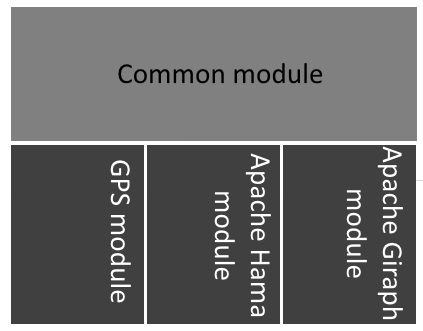
\includegraphics{arq_idea.png}}%\\
  \label{arq_idea}
\end{figure}

\section*{ Calendariza��o}
O novo planeamento para o projeto � o seguinte:
\begin{table}[h]
 \caption{ Calendariza��o semanal}
 \begin{tabular}{|l|l|p{9.5cm}|}
 \hline
 \bf{Data de Inicio} & \bf{Semana} & \bf{Descri��o} \\ \hline
 3 Mar�o & 1 & Escrita da Proposta \\ \hline
 10 Mar�o & 2 & Finaliza��o da Proposta e inicia��o do estudo das Plataformas \\ \hline
 17 Mar�o & 3 & Estudo das Plataformas e levantamento das interfaces program�veis. \\ \hline
 22 Mar�o & 4 & Estudo dos algoritmos \textit{k-core}, \textit{heat kernel} e \textit{BFS}  \\ \hline
 31 Mar�o & 5-6 & Estudo dos algoritmos \textit {Layered Label Propagation} e \textit{Louvain}. Estruturar e implementar os v�rios m�dulos da biblioteca.\\ \hline
 14 Abril & 7 & Continua��o da estrutura��o e implementa��o dos m�dulos da biblioteca.\\ \hline
 21 Abril & 8 & Implementa��o dos algoritmos estudados na 4� semana. Relat�rio de progresso.\\ \hline
 28 Abril & 9 & Prepara��o da apresenta��o individual e relat�rio de progresso. \\ \hline
 5 Maio & 10 & Continua��o da implementa��o dos algoritmos estudados na 4� semana. In�cio da implementa��o dos algoritmos \textit{Louvain} e \textit{Layered Label Propagation}.
 12 Maio & 11-12 & Continua��o da implementa��o dos algoritmos \textit{Louvain} e \textit{Layered Label Propagation}.\\ \hline
 26 Maio & 13-14 & Estudar e implementar o algoritmo de \textit{Betweenness Centrality}. \\ \hline
 9 Junho & 15 & Cartaz e finaliza��o da vers�o com a implementa��o dos algoritmos obrigat�rios. \\ \hline
 16 Junho & 16-19 & Escolha dos \textit{data-sets} (que iram ser usados nos testes), testes e compara��es com outras plataformas. \\ \hline
 14 Julho & 20 & Finaliza��o do relat�rio e entrega da vers�o final. \\ \hline
\end{tabular}
\end{table}
\\[0.5cm]
Devido a problemas inesperados foi necess�ria uma semana extra para a estrutura��o e implementa��o dos m�dulos da biblioteca.
A calendariza��o entregue na proposta tinha um erro nas semanas 9-10 onde o grupo tinha dado duas semanas para a prepara��o da apresenta��o individual e relat�rio de progresso quando na verdade existia apenas uma. Isto levou a uma semana extra ap�s a entrega, a semana 10.

\newpage

% REFERENCIAS
%
% Se utilizarmos BibTeX:
% \bibliographystyle{}
% \bibliography{}
%
% Caso contr�rio:
\begin{thebibliography}{99.}

\bibitem{louvain} Blondel, Vincent D., et al. "Fast unfolding of communities in large networks." Journal of Statistical Mechanics: Theory and Experiment 2008.10 (2008): P10008.

\bibitem{llp} Boldi, Paolo, et al. "Layered label propagation: A multiresolution coordinate-free ordering for compressing social networks." Proceedings of the 20th international conference on World Wide Web. ACM, 2011.

\bibitem{hama} Apache Hama. https://hama.apache.org/.

\bibitem{giraph} Apache Giraph. https://giraph.apache.org/.

\bibitem{hadoop} Apache Hadoop. http://hadoop.apache.org/.

\bibitem{docgps} Salihoglu, Semih, and Jennifer Widom. "Gps: A graph processing system." Proceedings of the 25th International Conference on Scientific and Statistical Database Management. ACM, 2013.

\bibitem{bspanalisys} Redekopp, Mark, Yogesh Simmhan, and Viktor K. Prasanna. "Optimizations and Analysis of BSP Graph Processing Models on Public Clouds." Parallel \& Distributed Processing (IPDPS), 2013 IEEE 27th International Symposium on. IEEE, 2013.

\bibitem{pregel} Malewicz, Grzegorz, et al. "Pregel: a system for large-scale graph processing." Proceedings of the 2010 ACM SIGMOD International Conference on Management of data. ACM, 2010.
 
%\bibitem{bc} Brandes, Ulrik. "On variants of shortest-path betweenness centrality and their generic computation." Social Networks 30.2 (2008): 136-145.
\bibitem{bc} David A. Bader, Shiva Kintali, Kamesh Madduri, and Milena Mihail. Approximating
betweenness centrality. In
Proc. 5th Workshop on Algorithms and Models for the Web
Graph, pages 124-137, 2007.

\bibitem{heatkernel} Chung, Fan. "The heat kernel as the pagerank of a graph." Proceedings of the National Academy of Sciences 104.50 (2007): 19735-19740.

%\bibitem{kcore} Dorogovtsev, Sergey N., Alexander V. Goltsev, and Jose Ferreira F. Mendes. "K-core organization of complex networks." Physical review letters 96.4 (2006): 040601.
\bibitem{kcore} Fortunato, Santo, and Marc Barthelemy. "Resolution limit in community detection." Proceedings of the National Academy of Sciences 104.1 (2007): 36-41.

\bibitem{bsp}Valiant, Leslie G. "A bridging model for parallel computation." Communications of the ACM 33.8 (1990): 103-111.

\bibitem{bfs} Edward F. Moore. The shortest path through a maze. In Proceedings of the International
Symposium on the Theory of Switching, pages 285-292. Harvard University Press, 1959.

\end{thebibliography}

\end{document}





